\documentclass{standalone}
 
\usepackage{pgfplots}
\usepackage{txfonts}
\pgfplotsset{compat = newest}
 
\begin{document}

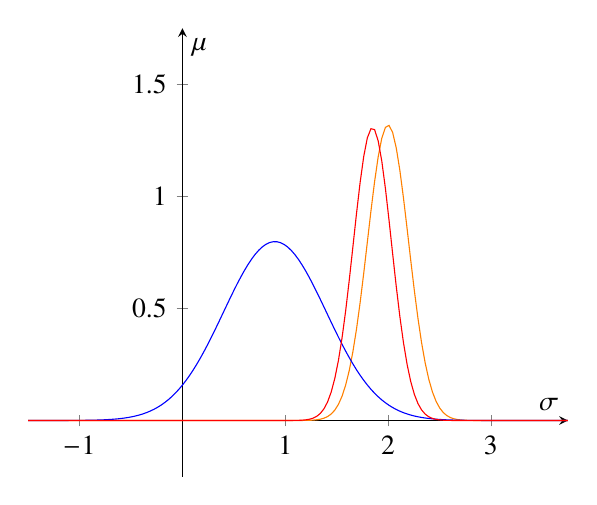
\begin{tikzpicture}[>=latex,thick]


\begin{axis}[
    xmin = -1.5, xmax = 3.75,
    ymin = -0.25, ymax = 1.75,
    axis lines = center,
    xlabel = $\sigma$,
    ylabel = {$\mu$},
]

\addplot [
    domain=-2:5, 
    samples=200, 
    color=orange,
]
{(1/(2*pi*0.2^2)^0.2)*exp(-(x-2)^2/(2*0.2^2))};

\addplot [
    domain=-2:5, 
    samples=200, 
    color=blue,
    ]
    {1/(2*pi*0.5^2)^0.5)*exp(-(x-0.9)^2/(2*0.5^2))};
    
\addplot [
    domain=-2:5, 
    samples=200, 
    color=red,
    ]
    {((1/(2*pi*0.5^2)^0.5)*exp(-(x-0.9)^2/(2*0.5^2))*(1/(2*pi*0.2^2)^0.2)*exp(-(x-2)^2/(2*0.2^2)))/0.1};


\end{axis}
\end{tikzpicture}


\end{document}
